\documentclass[technical_document.tex]{subfiles}
Object avoidance is done using ultrasone sensors. Eva has 6 ultrasone sensors at the front, two sensors scanning backwards and one sensor to each side. See figure \ref{fig:ultra_sensors} Depending on where an object is detected with the ultrasone sensors, the speed of the left or right wheel will be scaled down, so Eva will avoid the object. The scaling will have more effect when the measured distance to the object is small and will have less effect if the distance is large.

The following example gives more insight in how this method works. If the ultrasone sensors on the front left detect an object, then the right wheel will go slower, making Eva turn right. The same goes for the side sensors when an object is detected on the sides, for the front sensors in the middle etc.

Since the sides only have one sensor each, avoiding objects on the sides is easy. Eva simply needs to turn right when something on the left is detected and turn left whenever something on the right is detected. Also, because Eva won't drive backwards while going to her goal (only when she needs to adjust her position in front of a table), the sensors at her back are only used to stop the wheels when something is detected. 

The following formula is used by the sensors on the side to scale the speeds of the wheels:

\begin{equation*}
scaled\_speed = min(speed, \frac{speed-speed * (avoidance\_distance-measured\_distance)}{avoidance\_impact})
\end{equation*}

Where:
\begin{itemize}
\item speed is the reference speed to be scaled down;
\item avoidance\_distance is the distance needed before the scaler takes effect;
\item avoidance\_impact is the degree to which the scaler has effect;
\item measured\_distance is the measured distance by one of the sensors in a unit;
\end{itemize}

The sensors on the front, however, are used in a more complicated way.
Since there are six sensors in front, detecting objects happens with more accuracy. Eva uses three units consisting of two sensors each and uses these units to calculate the scaling for the left or right wheel.

\newpage
The following formula is used by a unit at the front to scale the speeds of the wheels:

\begin{equation*}
scaled\_speed = min(speed, min(\frac{speed-speed * (avoidance\_distance-measured\_distance1)}{avoidance\_impact}
\end{equation*}

\begin{equation*}
, \frac{speed-speed * (avoidance\_distance-measured\_distance2)}{avoidance\_impact}))
\end{equation*}
Where the same parameters are used as the side sensors, except that the measured distance of another sensor (the other sensor in a unit) is used in the calculations as well.

\begin{figure}[ht!]
	\centering
	\mbox{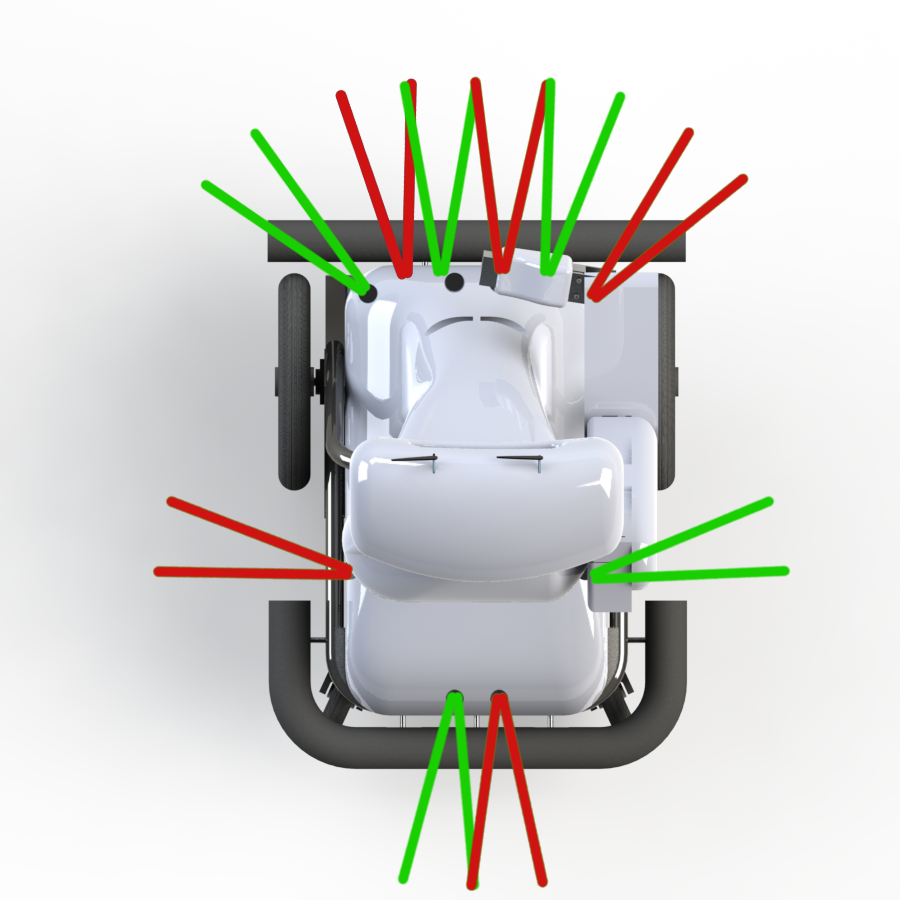
\includegraphics[scale=1]{Images/eva_topView_sensors.png}}
	\caption{Ultrasone sensors of Eva. The green sensors will emit ultrasonic waves together, the same holds for the red sensors.}
	\label{fig:ultra_sensors}
\end{figure}